In chapter 6 we described the theoretical aspect behind our implementation and doing so described the architectural design of the implementation. In this chapter we describe how we have implemented the design, which challenges we have encountered doing so. We will also be looking at the performance and security of the implementation.


\section{Introduction}




\section{Implementing the application}



\subsection{Design and Implementation}

\begin{figure}[H]
    \centering
    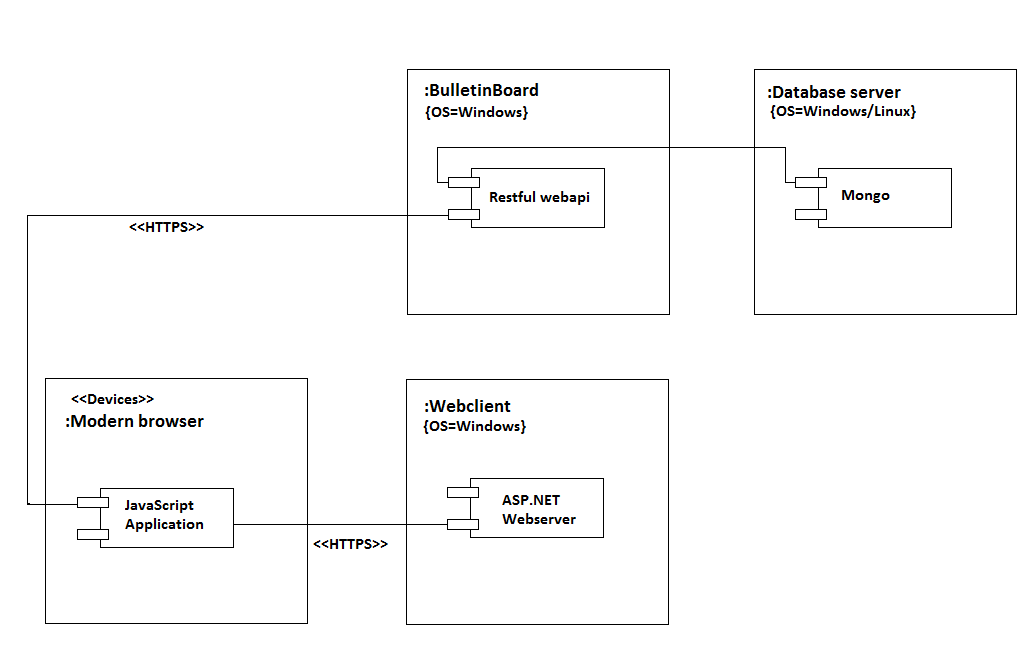
\includegraphics[scale=0.50]{Deployment_view.png}
    \caption{Final deployment view}
\end{figure}




\section{Analyzing the implementation}
We will in this section analyze of implementation. We will analyze the chosen tactics, the code quality and evaluate the security in the implementation. 

\subsection{Security analyze}
In Section \ref{sec:security_requirements} several security requirements that a secure 
and complete cryptography voting protocol should satisfy where listed. We will look at
these requirements and see if our implementation satisfy these. We will also 


\subsubsection{Generating Prime}

\subsubsection{Generating Prime}
Generating very large primes is a computationally hard task and thous time consuming. Given the fact
that the prime $q$ used in our implementation is public known, it is easy to think that one could simply
use one or a set of very large hardcoded primes. However, by performing a large precomputation for a given
prime an adversary can quickly calculate arbitrary discrete logarithms in that group, efficiently reducing 
computation cost for all targets that uses this group \cite{Adrian:2015:IFS:2810103.2813707}. 



\subsubsection{Electronic voting secure requirements}

\begin{description}
    \item[Voter Privacy]
        No one should be able to link a vote back to the specific voter, and only the voter should
        know his vote. These requirements shall hold during and after the election.  
        
        This requirement is meet by our implementation, infact its one of the core elements in the
        Election voting protocol from section \ref{sec:the_protocol}. Every voter only publish his vote
        though $U = G^{v+s}$ where $G$ is a generator and $v \in \{0,1\}$ and $s \in \Z_q$. As $s$ is only
        known by the voter and is uniformly random picked then the sum of $s$ and $v$ is also unknown for any 
        potential adversary under the security of the DL problem. And one could ague that even if an
        adversary should be break the DL problem then, unless he knows $s$, the vote $v$ would still
        be unknown. 
        
        
    \item[Eligibility]
        Unlike Voter Privacy, this requirement of non-eligible voters not being able to vote is not
        fulfill by the protocol it self. We handle this in our implementation though the registration service
        describe in section \textcolor{red}{[???]}. This enable us to change the registration service 
        accordingly to the nature of the election.         
        
        
    \item[Uniqueness]
        Uniqueness is about making sure only one vote is counted for each eligible
        voter. 
        
    \item[Fairness]
        To ensure all participants get a fair election, no partial tally must be
        revealed before the end of the voting. This is achieved in our implementation
        by only starting the tally phase when all votes are casted or when a deadline is 
        reached and the ballot casting phase ends. The Talliers in notified only by the Bulletinboard
        when to start the tally phase thou none other have the authority to do so.  
        
        Through the property of secret sharing used in the protocol, the secret to decrypt the
        vote is shared amoungst three or more talliers. These shares are again encrypted with the public key 
        of the corresponding tally. As a consequence, no one except the tally with the corresponding
        private key is able to decrypt the share.
        
        
         
    \item[Uncoercibility]
        Participating voters are able to vote freely, without anyone able to coerce
        them into casting a vote in a particular way. In addition, no authority should be able to extract the value of a vote.
        
    \item[Receipt-freeness]
         The voting system should not produce a receipt that reveals any information about the casted vote. This is to prevent a vote from trading his vote. 
         Our implementation only confirms the success of a voting, not the value of the vote. There is no functionality that enables any participants nor observers to
         gain information about the value of a vote. 
         
        
    \item[Accuracy]
        The final tally should be correctly computed from valid casted votes. It should not be
        possible to manipulate the final tally without being detected. \\
        
        \noindent
        Our implementation utilizes the proofs from the protocol to fulfill this requirement. 
        
        \noindent
        Under the Ballot casting phase of the protocol, we require that the voters proofs the correctness of there votes. This is done though the $Proof_U$ and $DLEQ$ proofs, which is required to be published along side the encrypted vote $U$. Should one of the proofs fail, then the vote is marked invalid and this vote is ignore in the preceding processes. 
        
        \noindent
        In the tally phase of the protocol, the tally multiplies its shares and then decrypts them and publishes the end result. Along with this result we require that the $DLEQ$ proof is published aswell. This allows us to verify the correctness of the tallying process for each tallier. Should a $DLEQ$ proof from a tallier fail then the tally's shares is ignore in the preceding process. The protocol requires the shares from at least $t$ talliers, in order to extract and calculate the end result. Should it 
        be the case that this requirement is not fulfill an re-election is require but untill then the implementation simply ignores the shares from the tally in question.
        
        \noindent
        Should an adversary gain access to the database serving the BulletinBoard, it would be possible for this adversary to manipulate the verdict of a proof but not
        the proofs them self, as the construction of the proofs prevent this. Thou our implementation does not take this scenario into account it would be fairly easy to make
        a functionality that reevaluates the proofs should such a breach have been detected. One could argue that an adversary with full access to the database could also remove elements such as a casted vote or the information that a given voter have voted. The later would effectually enable the given voter the ability to double vote, this scenario is not handled in our implementation. The first scenario is also possible but given the fact that our implementation have voter privacy and the votes is secure under the DL problem then the adversary would not know if he is removing and "no" or a "yes" vote. 
        
        
    \item[Universal Verifiability]
        It should be possible for any participants and observers to validate individual votes as well as the final tally of the election. 
        
        \noindent
        The protocol is basically designed around this requirement and as such most of the information is published to the Bulletinboard, and as describe under the requirement "Accuracy" our implementation requires both the voters and the talliers to publish proof of the correctness and the consistency of the vote and the shares to the BulletinBoard. 
        
        \noindent
        Everything on the BulletinBoard is publicly available both for participants and none participants of the election. $Proof_U$ verifies that an encrypted vote $U$ is either 0 or 1 and the DLEQ proofs verifies the consistence of the shares for both the voters and the talliers. The end result can be calculated from the publicly known information available after the tallying phase. 
            
    \item[Individual Verifiability]
        Every registered voter should be able to verify that his vote is counted correctly. 
        
        \noindent
        in our implementation there is no link between a vote and a voter when the  
        
        It would be desirable if a voter could be able to check that his encrypted vote
was counted and tabulated correctly in the final tally. The problem is that
the combination of receipt-freeness and individual verifiability requirements
obviously conflict with each other. One would need some kind of receipt in
order to achieve verifiability, but then the same receipt could be used for
vote buying or selling. As a consequence this voting application has given
preference to receipt-freeness and thus no functionality for verifying votes
later in the process are implemented.
        

\end{description}

